%% Support sites:
%% http://www.michaelshell.org/tex/ieeetran/
%% http://www.ctan.org/pkg/ieeetran
%% and %% http://www.ieee.org/

\documentclass[conference]{IEEEtran}
\usepackage{lipsum}
\usepackage{graphicx}
\usepackage{amsmath}
\usepackage{array}
\usepackage{url}


% correct bad hyphenation here
\hyphenation{op-tical net-works semi-conduc-tor}

% adjust spaces in asmath userpackage
\interdisplaylinepenalty=2500

\begin{document}
\title{Convex Optimization for \\Holistic Mechatronic System Design}

%%%%%%%%%%%%%% begin authors %%%%%%%%%%%%%% 
\author{\IEEEauthorblockN{Yuchao Li}
\IEEEauthorblockA{School of Mechanic and \\Mechatronic Engineering\\
Royal Institute of Technology\\
Stockholm, Sweden\\
Email: Yuchao@kth.se}
\and
\IEEEauthorblockN{Anqing Duan}
\IEEEauthorblockA{School of Mechanic and \\Mechatronic Engineering\\
Royal Institute of Technology\\
Stockholm, Sweden\\
Email: Anqingd@kth.se}
\and
\IEEEauthorblockN{Alexander Gratner}
\IEEEauthorblockA{School of Mechanic and \\Mechatronic Engineering\\
Royal Institute of Technology\\
Stockholm, Sweden\\
Email: Gratner@kth.se}}
%%%%%%%%%%%%%% end authors %%%%%%%%%%%%%%%%

\maketitle %\IEEEpeerreviewmaketitle

%%%%%%%%%%%%%% abstract %%%%%%%%%%%%%
\begin{abstract}
\lipsum[1]
\end{abstract}
%%%%%%%%%%%%%% end abstract %%%%%%%%%%%%%%%

%%%%%%%%%%%%%% begin introduction %%%%%%%%%
\section{Introduction}

% Designing mechatronic systems is a problematic task.. 
% These persons has therefore made significant contributions
% Bond Graph approach
% Genetic algorith approach
% Some other methodologies
% Accordning to this book, convex is better..
% Introducing convex optimization would go a long way in solving the design dilemma..



Could the current resaerch trend of using genetric algorithms as a solver of mechatronic design optimization problems be improved by adapting a diciplinary convex optimization approach? The multidiciplinary nature of mechatronic systems, which could be characterised as systems with synergetic integrations of mechanical engineering with eletronics and intelligent computer control \cite{harashima1999}, makes early design optimization a difficult process. Optimizations are often done in the latter detailed design phases \cite{(I CEDEX) Engineering design; A systematic approach, 3rd ed} whereas early design decisions becomes a limiting factor. Research on the topic of optimization in early design stages for mechatronic systems has presented both holistic and non-holistic approaches which share the common feature of using genetic algorithms, either as a complement or as a standalone solver. The disadvantages of GA when it comes to accuracy and computation time justifies research on applying diciplinary convex optimization.

\par
%Modern research within the field of mehcatronic systme optimization has...
Optimizing mechatronic systems using genetic algorithms has been widely explored by researchers today. Hammadi \cite{Hammadi} proposes an emergent multi-agent approach where the system is decoposed into smal sub-systems (or agents) that in turn is optimized using the genetic algorithms NSGA II. Another approach that uses NSGA II is proposed by Guizani \cite{GUizani} where a partioning method is utilized to decompose the mechatronic system and classification of the interactions between partions are done. An approach developed by Seo \cite{Seo} and further developed by Behbahani \cite{Behabani} uses a two loop optimization process which incorperates genetic algorithms and bond graphs in an outer loop to otimize system topology and genetic programming in an inner loop to fin the elite solution within the optimal topology. The research in this paper will be based upon the work done by Malmquiest et al. \cite{Malmquist} where they created a framework named IDIOM which optimizises mechatronic systems in a holistic manner by the use of genetic algorithms.

\par

The IDIOM framework developed by Malmquist et al. extends on the Roos \cite{Roos} on a research on a methodology for integrated design och mechatronic servo systems. In his research, Roos reflects on the choice of using genetic algorithms to optimize the servo systems by stating that "The drawback of this method for system optimization is that it is computationally intensive and that there exists no mathematical proof that it actually finds the true optimum". This statement justifies the exploration of other optimization techniques which could provide true optimizations in a less computationally intensive manner, and for which convex optimization has been chosen. Diciplinary convex programming is a methodology developed by Grant et al. \cite{Grant} which purpose, according to the authors, is to "allow much of the manipulation and transformation required to analyze and solve convex programs to be automated". The methodology originates from procedures taken by those who regularly study convex optmization problems and has been implemented in the modelling framework called CVX \cite{CVX}.  

\par
The argument made by Roos serve as a starting point in the research presented in this report. It challenges the current trend of using evolutionary algorithms when optimizing the design of mechatronic systems and could provide a optimization approach that is less compututionally expensive and more accurate. 

\par
The remainder of this paper will introduce the prevuous work done by Malmquist et al. of which this study aim to extend on. \$3 describes the method used when applying convex optimization to the mechatronic system. Finally, \$4 introduces a case study where a system optimization is performed, and compared to the results obtained by Malmquist et al.  , of a mechatronic system composed of a motor, planetary gear and a load.  


%Mechatronic systems can be characterised as systems that emphasize on the synergetic integration of mechanical engineering with electronics and intelligent computer control \cite{harashima1999}. This multidiciplinary nature of the systems makes early design optimization difficult which is why most optimization processes today are done in the latter detailed design phase \cite{Cedex2014}. However, these optimization processes become limited by early design decisions and are therefore not resulting in a truly optimal system. Previous research on the topic of early design optimization in mechatronic systems has presented various approaches whereas the majority utilizes evolutionary algorithms (such as genetic algorithms), either as complement or as a standalone optimization technique. Disadvantages when optimizing with GAs is that the method does not necessary find the optimal point and that response time become large when the parameter space increases \cite{Boyd}. These problems justifies a different optimization method, such as convex optimization, to be applied. 

%A disadvantage when optimizing with GAs is that the approach does not necessary produce the most optimal solution and the that the computational time increases a lot when applying it on complex systems.    

%Previous research has presented methodologies to solve this early design optimization. 

%A lot of methodologies has been presented within the field 

%An aspect shared by the majority of them


%The majority of approaches..


%optimizations done in the latter design stages are limited by early design decisions and are therefore not generating an truly optimal system.  
%a
%and this process is often done in later, detailed design phases \cite and the optimization is therefore constrained by design choices in early stages. Approaches or methodologies to solve this problem in early design phases. 

%FUNKAR DET?

%This section should include:
%\begin{enumerate}
%\item Problem statement
%	\subitem Emphasize (Justify that the problem is important)
%\item Analyze the gap (specific, technical)
%\item What will you do to fill the gap.
%\item Summarize contributions (Summarize step 1-3, emphasize on 1.2)
%\item Outlook of structure. 
%\end{enumerate}

%%%%%%%%%%%%%% end introduction %%%%%%%%%%%

%%%%%%%%%%%%%% begin conclusion %%%%%%%%%%%
\section{Conclusion}
Conclusion ehhase
%%%%%%%%%%%%%% end conclusion %%%%%%%%%%%%%

%%%%%%%%%%%%%% begin acknowlegement %%%%%%%
\section*{Acknowledgment}
%%%%%%%%%%%%%% end acknowlegement %%%%%%%%%

%%%%%%%%%%%%%% begin acknowlegement %%%%%%%
\begin{thebibliography}{1}

\bibitem{IEEEhowto:kopka}
H.~Kopka and P.~W. Daly, \emph{A Guide to \LaTeX}, 3rd~ed.\hskip 1em plus
  0.5em minus 0.4em\relax Harlow, England: Addison-Wesley, 1999.

\end{thebibliography}
%%%%%%%%%%%%%% end acknowlegement %%%%%%%%%

\end{document}



%\section*{Handy Examples}

%\subsection*{Figure example}

%\begin{figure}[!t]
%\centering
%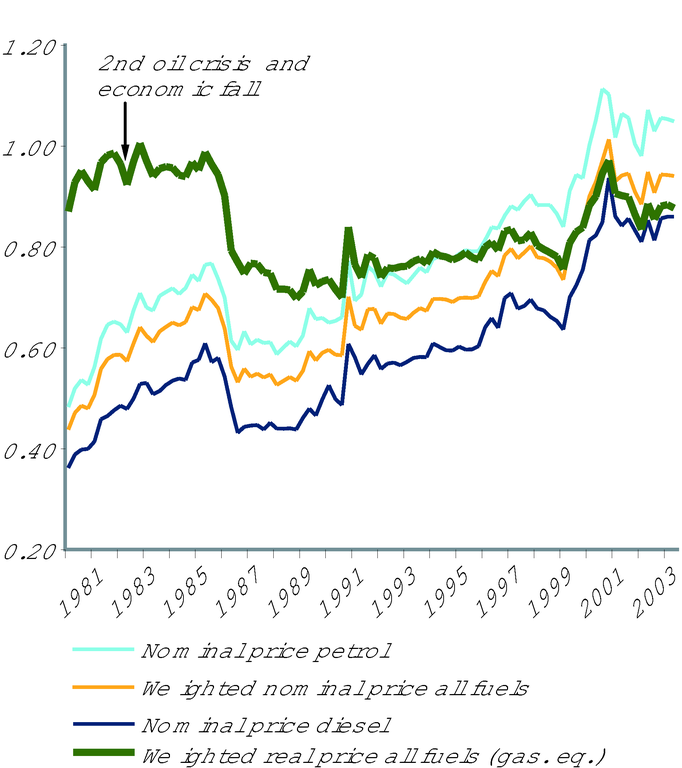
\includegraphics[width=0.25\textwidth]{./Contents/myFigure.png}
%\caption{Simulation results for the network.}
%\label{fig_sim}
%\end{figure}

%\subsection{Table example}
%\begin{table}[!t]
%% increase table row spacing, adjust to taste
%\renewcommand{\arraystretch}{1.3}
% if using array.sty, it might be a good idea to tweak the value of
% \extrarowheight as needed to properly center the text within the cells
%\caption{An Example of a Table}
%\label{table_example}
%\centering
%% Some packages, such as MDW tools, offer better commands for making tables
%% than the plain LaTeX2e tabular which is used here.
%\begin{tabular}{|c||c|}
%\hline
%One & Two\\
%\hline
%Three & Four\\
%\hline
%\end{tabular}
%\end{table}




